% Modified for use with JCC - Madhusudan Singh Copyright (C) (2012). All rights reserved.
\documentclass[12pt]{article}

\setlength{\oddsidemargin}{0in}  %left margin position, reference is one inch
\setlength{\textwidth}{6.5in}    %width of text=8.5-1in-1in for margin
\setlength{\topmargin}{-0.5in}    %reference is at 1.5in, -.5in gives a start of about 1in from top
\setlength{\textheight}{9in}     %length of text=11in-1in-1in (top and bot. marg.) 
\newenvironment{wileykeywords}{\textsf{Keywords:}\hspace{\stretch{1}}}{\hspace{\stretch{1}}\rule{1ex}{1ex}}

\usepackage{amsmath,amssymb}
\usepackage{graphicx}% Include figure files
%\usepackage{caption}
\usepackage{color}% Include colors for document elements
\usepackage{dcolumn}% Align table columns on decimal point
%\usepackage{bm}% bold math
\usepackage[numbers,super,comma,sort&compress]{natbib}
%\usepackage[nolists, nomarkers, figuresfirst]{endfloat}
\usepackage{subfig}
%\usepackage{booktabs}
\usepackage{longtable}

\definecolor{background-color}{gray}{0.98}

\title{istar: A Novel Web Platform for Large-Scale Online Protein-Ligand Docking}
\author{Hongjian Li, Kwong-Sak Leung and Man-Hon Wong\thanks{The authors are with Department of Computer Science and Engineering, Chinese University of Hong Kong}}

\begin{document}

\maketitle

\begin{abstract}
We are motivated by the desire to automate large-scale protein-ligand docking for drug discovery using our docking engine idock and thus have developed a novel web platform called istar. Without tedious software installation, users, especially computational chemists, can submit jobs on the fly either by using our web site or by programming against our RESTful API. Our HTML5- and CSS3-powered istar web site supports 1) filtering ligands by desired molecular properties and previewing the number of ligands to dock, 2) monitoring job progress in real time, and 3) outputting predicted free energy, ligand efficiency, putative hydrogen bonds, and supplier information for easy purchasing, three unique and useful features commonly lacked on other online docking platforms like DOCK Blaster or iScreen. We have collected 12,171,187 yuck-free ligands from the clean subset of the ZINC database with conditional permission from its developer. We have revamped our docking engine idock to version 2.0, further improving docking speed and accuracy, inventing new functionalities, and fixing bugs. To better evaluate and compare idock 2.0 with the state-of-the-art AutoDock Vina 1.1.2, we have carried out a redocking benchmark on the 2,897 and 2,455 protein-ligand complexes of the refined set of PDBbind v2012 and v2011 respectively and 343 protein-ligand complexes of CSAR NRC HiQ Set 24Sept2010, and a virtual screening benchmark on 12 diverse proteins and 3000 ligands of different molecular weight. The results have shown that under various circumstances idock displayed comparable success rates but outperformed AutoDock Vina in terms of docking speed by at least 8.69 times and at most 37.51 times, making idock particularly suitable for large-scale protein-ligand docking. We have developed a customized daemon from idock 2.0 on istar, implementing our novel idea of two-phase docking, and exploiting both fine-grained slice-level parallelism in phase 1 and coarse-grained job-level parallelism in phase 2 in order to further shorten job execution time, as well as using gzip to compresses result files in order to save server storage and network bandwidth. We have prepared two graphical tutorials for novices to get started easily. We have tested our istar web site successfully in Chrome 19+, Firefox 12+, IE 9+, Safari 5+ and Opera 12+. We aim to make istar into a large-scale online docking platform really pragmatic for the computational chemistry community and pharmaceutical companies.
\end{abstract}

\begin{wileykeywords}
docking, virtual screening, web.
%A list of five key words or phrases which best characterize the paper are required for indexing.
\end{wileykeywords}

\clearpage

%*****************Graphical Table of Contents******************** THIS IS MANDATORY *******************


\begin{figure}[h]
\centering
\colorbox{background-color}{
\fbox{
\begin{minipage}{1.0\textwidth}
%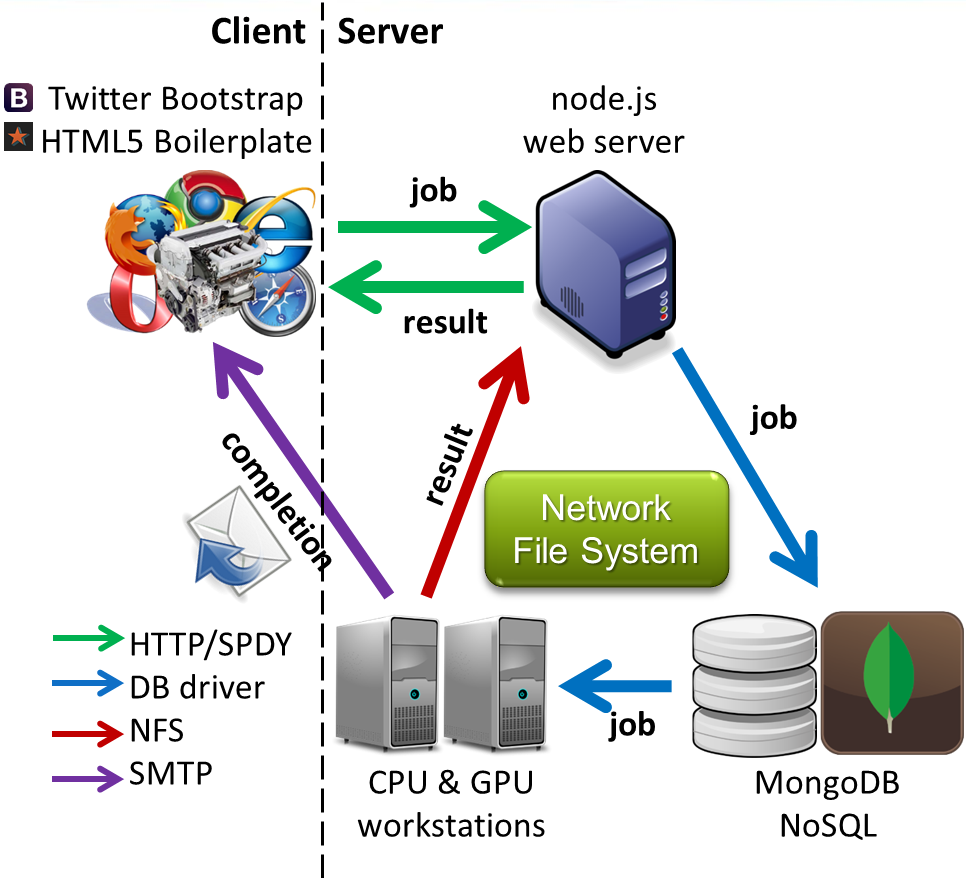
\includegraphics[width=55mm,height=50mm]{GTOC.png} % Pick only one of the two styles by uncommenting the corresponding \includegraphics
%\\
We are motivated to automate large-scale protein-ligand docking using our docking engine idock and thus have developed a novel web platform called istar. Without tedious software installation, users can submit jobs on the fly either by browsing our web site or by programming against our RESTful API. Our HTML5- and CSS3-powered istar web site supports several unique and pragmatic features that cannot be found on other online docking platforms.
\end{minipage}
}}
\end{figure}

% makes references listed with 1., 2., etc.  
  \makeatletter
  \renewcommand\@biblabel[1]{#1.}
  \makeatother

\bibliographystyle{apsrev}

\renewcommand{\baselinestretch}{1.5}
\normalsize


\clearpage


\section*{\sffamily \Large SUMMARY}

We have developed istar, a novel web platform for large-scale online protein-ligand docking for drug discovery. Without tedious software installation, users can submit jobs on the fly either by using our web site or by programming against our RESTful API. Our HTML5- and CSS3-powered istar web site supports 1) filtering ligands by desired molecular properties and previewing the number of ligands to dock, 2) monitoring job progress in real time, and 3) outputting predicted free energy, ligand efficiency, putative hydrogen bonds, and supplier information, three very useful features commonly lacked on other online docking platforms like DOCK Blaster \citep{557} or iScreen \citep{899}. We have collected 12,171,187 yuck-free ligands from the clean subset of ZINC \citep{532,1178} with conditional permission from its developer. We have revamped our docking engine idock \citep{1153} to version 2.0, further improving docking speed and accuracy, inventing new functionalities, and fixing bugs. We have developed a customized daemon from idock 2.0 on istar, implementing two-phase docking and exploiting fine-grained slice-level parallelism in order to further shorten job execution time, as well as using gzip to compresses result files in order to save server storage and network bandwidth. We have also prepared two graphical tutorials for novices to get started easily. We have tested our istar web site successfully in Chrome 19+, Firefox 12+, IE 9+, Safari 5+ and Opera 12+. We aim to make istar a large-scale online docking platform really pragmatic for the computational chemistry community and pharmaceutical companies.

\section*{\sffamily \Large INTRODUCTION} % Not needed for rapid communications

Protein-ligand docking predicts the preferred conformation and binding affinity of a small ligand when it is non-covalently bound to a specific binding site of a macro protein. Up to date, there are hundreds of docking programs \citep{493,922}. The AutoDock series is the most cited docking software in the research community. AutoDock has contributed to the discovery of several drugs, including the first clinically approved HIV integrase inhibitor \citep{1169}. Technically speaking, AutoDock is single threaded \textit{per se}. Following its initial release, several parallel implementations were developed, using either multithreading or computer cluster \citep{115,560,782}.

In 2009, AutoDock Vina \citep{595} was released. As the successor of AutoDock 4 \citep{596}, AutoDock Vina significantly improves the average accuracy of the binding mode predictions while running two orders of magnitude faster with multithreading \citep{595}. It was compared to AutoDock 4 on selecting active compounds against HIV protease, and was recommended for docking large molecules \citep{556}. Its functionality of semi-flexible protein docking by enabling flexibility of side-chain residues was evaluated on VEGFR-2 \citep{1084}. To further facilitate the usage of AutoDock Vina, auxiliary tools were subsequently developed, including a PyMOL plugin for program settings and visualization \citep{609}, a bootable operating system for computer clusters \citep{773}, and a GUI for virtual screening on Windows \citep{1250}. AutoDock Vina is free and open source. So far it has been cited by over 500 publications according to Google Scholar, making it a very competitive docking program.

In 2011, inspired by AutoDock Vina, we developed idock 1.0 \citep{1153}, a multithreaded virtual screening tool for flexible ligand docking. idock inherits from AutoDock Vina the accurate scoring function and the efficient optimization algorithm, and meanwhile introduces a fruitful of innovations, such as receptor and grid map caching for efficient large-scale virtual screening, revised numerical model for much faster energy approximation, capability of automatic detection and deactivation of inactive torsions for dimensionality reduction, utilization of our lightweight thread pool to parallelize grid map creation and reuse threads, utilization of the new C++11 feature of right-value references to avoid frequent memory reallocation, and accelerated parsers for both receptors and ligands. When benchmarked on docking 10,928 drug-like ligands against HIV reverse transcriptase, idock 1.0 achieved a speedup of 3.3 in terms of CPU time and a speedup of 7.5 in terms of elapsed time on average compared to AutoDock Vina.

Having released idock, we kept receiving docking requirements from our colleagues and collaborators. They are mostly biochemists and pharmacists, outsourcing the docking research to us after discovering pharmaceutical protein targets for certain diseases of therapeutic interest. Consequently, we had to grab the protein structure, do format conversion, define search space, set up docking parameters, and keep running idock in batch for months. Tedious enough, all the above work was done manually, resulting in very low research productivity. In order to automate large-scale protein-ligand docking using our idock, we have therefore developed a novel web platform called istar. Figure \ref{relationship} depicts the relationship between istar and idock. istar is a novel web platform while idock is a concrete application hosted on the istar platform.

There are other online protein-ligand docking platforms. DOCK Blaster \citep{557} investigates the feasibility of full automation of protein-ligand docking. It utilizes DOCK \citep{1222} as the docking engine and ZINC \citep{532,1178} as the ligand database. iScreen \citep{899} is a compacted web server for TCM (Traditional Chinese Medicine) docking and followed by customized \textit{de novo} drug design. It utilizes PLANTS \citep{610,607,779} as the docking engine and TCM@Taiwan \citep{528} as the ligand database. It also utilizes LEA3D \citep{1223} for \textit{de novo} ligand design. FORECASTER \citep{1012} is a web interface consisting of a set of tools for the virtual screening of small molecules binding to biomacromolecules (proteins, receptors, and nucleic acids). It utilizes the flexible-target docking program FITTED \citep{602} as docking engine. Nevertheless, the above platforms neither provide ligand selection based on molecular properties, nor display job progress in real time. They also lack straightforward output of compound suppliers, a hurdle preventing users from purchasing high-rank compounds for further wet-lab verification. Our istar platform has properly addressed the above obstacles.

Here is the outline of the paper. We will first describe the five functional components of istar, followed by its novel features that are only available on istar and commonly unavailable on other docking platforms. We will then present the key features of idock 2.0 compared to version 1.0. In the result section, we will detail the benchmarks and results of both redocking and virtual screening. Finally we will give software availability and a discussion.

\section*{\sffamily \Large ARCHITECTURE}

Figure \ref{architecture} shows the architecture of istar. There are five major components, a web site, a web server, a database management system, several workstations, and a network file system. Under typical circumstances, a user browses our web site and submits a job. The web server first validates user input and then saves it into the database. Several workstations keep running daemons in the background, fetching jobs from the database and carrying out experiments. Upon completion, they send a notification email to the user and write the result to the network file system, which is cached as static content by the web server. The user again browses our web site to download result or monitor job progress.

\subsection*{\sffamily \large Web Site}

We have seamlessly combined both the Twitter Bootstrap and the HTML5 Boilerplate into a HTML5- and CSS3-powered istar web site (Figure \ref{idock}). From top to bottom, the first section displays information about existing jobs, including the number of ligands to dock, submission date, current status and progress, and result for download upon completion; the second section allows new job submission by specifying a receptor, its search space, and optionally, desired ligands to dock; the third section plots the histogram distributions of 9 molecular properties of the 12 million ligands; the fourth section delivers two graphical tutorials for newbies to get started easily. We have tested the web site successfully in Chrome 19+, Firefox 12+, Internet Explorer 9+, Safari 5+ and Opera 12+.

A job typically comprises compulsory fields and optional fields. Compulsory fields include a receptor in PDBQT format, a search space defined by a cubic box, a short job description, and an email to receive completion notification. Optional fields include 9 ligand filtering conditions, which are molecular weight, partition coefficient xlogP, apolar desolvation, polar desolvation, number of hydrogen bond donors, number of hydrogen bond acceptors, topological polar surface area tPSA, net charge, and number of rotatable bonds (Figure \ref{LigandProperties}), in the form of closed intervals. We set up the default values of lower and upper bounds for the 9 molecular properties. Only the ligands satisfying all the 9 filtering conditions will be docked. In order to nullify a specific filtering condition, one may expand its closed interval to cover the entire possible range because of the relationship of logical and.

We have prepared two graphical tutorials for users to correctly fill in the compulsory fields. Tutorial 1 illustrates how to prepare a receptor in PDBQT format with MGLTools \citep{596}. Tutorial 2 illustrates how to define a search space with MGLTools \citep{596}, Chimera \citep{1219} or PyMOL \citep{1221}. We deliberately do not introduce an automatic protein binding site detection tool but let the graphical tutorials guide this process with full customization.

\subsection*{\sffamily \large Web Server}

We have built the web server using the high-performance express.js web application framework on top of the asynchronous event-driven node.js engine. In addition to the conventional HTTP 1.x protocol, the web server also supports the SPDY protocol v3, the prototype of next generation HTTP 2.0, achieving reduced latency through compression, multiplexing, and prioritization.

We have developed a customized validator module to validate and sanitize user input upon new job submission. Users will be notified by tips should there be any validation errors, such as invalid receptor format, excessively small or excessively large search space, or invalid email address. Only valid jobs are saved into the database.

\subsection*{\sffamily \large Database}

We have established the database using MongoDB, a scalable, high-performance, open source NoSQL database. MongoDB features document store in JSON (JavaScript Object Notation) style, making it particularly suitable for applications requiring flexible document attributes like our istar. 

\subsection*{\sffamily \large Workstations and Daemons}

We have deployed several workstations to simultaneously run a customized idock daemon in the background. We have derived the daemon from idock 2.0, adding dozens of lines of code to iteratively and atomically fetch a pending job from MongoDB, reuse the receptor structure and grid maps whenever possible, perform 2-phase docking, exploit 2-level parallelism, report progress to MongoDB, output verbose information, and send email notification upon job completion. We have further improved idock to version 2.0 in terms of docking speed and accuracy, new functionalities, and bugfixes.

\subsection*{\sffamily \large Network File System}

We have configured a network file system for shared access from the workstations, the web server, and the database server. Onto the network file system, we have collected and saved 12,171,187 clean ligands at pH 7 in mol2 format from the ZINC database \citep{532,1178} with explicit permission of its major developer and maintainer, Prof. John J. Irwin at University of California, San Francisco. Originally the yuck-compound-free ligands are organized into 98 slices, with each slice containing approximately 125,000 clean ligands, among which about 75,000 (60\%) have a molecular weight of at least 350g/mol, the minimum weight requirement that a modern drug should bear. We have converted the entire 12 million ligands into PDBQT format in batch, and combined the 12 million individual structures and their 9 molecular properties and supplier information into one single file as huge as 50GB. We have recorded and encoded the offset of each ligand for fast random seeking and parallel docking.

\section*{\sffamily \Large NOVEL FEATURES OF ISTAR}

We would like to highlight the novel and unique features that are only available on istar.

\subsection*{\sffamily \large Ligand Filtering}

istar supports filtering ligands by desired molecular properties and previewing the number of ligands to dock. This novel feature is achieved by inter-process message passing and in-memory table scan.

During web server startup, the master process loads the 9 molecular properties of the 12 million ligands into memory, and then forks worker processes, which await connections. Once a user changes any of the 9 filtering conditions on the web site, a new query is initiated and sent to the web server. One of the worker processes accepts the query and forwards it to the master process through inter-process message passing. The master process performs an in-memory table scan and aggregates the number of ligands satisfying all the 9 filtering conditions. The ligand count is then signaled back to the query-invoking worker process and then forwarded to the user on the web site. Such an entire round trip costs approximately one second, rendering the feasibility of real-time ligand counting for users to estimate in advance how many ligands will be docked.

Before docking a ligand, our idock daemon checks its 9 molecular properties against the 9 filtering conditions. If any condition fails, the daemon simply skips the current ligand and proceeds to the next one by looking up the offset table.

\subsection*{\sffamily \large Real-Time Progress}

istar supports monitoring job progress in real time. This novel feature is achieved by the progress reporting mechanism inside our idock daemon as well as our Ajax (Asynchronous JavaScript and XML) timer and table on the web site.

After docking a ligand, our idock daemon increments a counter and reports the progress to the database. When a user browses our istar web site, an Ajax timer is automatically started, querying against the web server for the most current progress of jobs of the same user at an interval of one second. If the job progress is updated, it is displayed in the corresponding table cell in an Ajax manner without page refresh. In this way, a user can always keep track of job progress in real time, especially for long-running jobs.

\subsection*{\sffamily \large Verbose Output}

Our idock daemon outputs verbose information to both docked PDBQT file (Figure \ref{OutputPDBQT}) and summary CSV (Comma-Separated Vector) file (Figure \ref{OutputCSV}).

The docked PDBQT file includes predicted free energy, inter-ligand free energy, intra-ligand free energy, ligand efficiency, putative hydrogen bonds, and per-atom inter-ligand free energy. Please refer to our idock 1.0 paper \citep{1153} for the mathematical equations of free energy evaluation in detail. By default, ligands are ranked in the ascending order of predicted free energy normalized by torsional degree of freedom. Alternatively, users can easily transit to other ranking options using derived efficiency indexes \citep{335,336,337}. The per-atom inter-ligand free energy facilitates detection of protein-ligand interaction hotspots, and helps improving ligand potency by altering certain chemical moieties while retaining those critical for binding.

The summary CSV file includes the ZINC ID, predicted free energy and ligand efficiency and putative hydrogen bonds of the top 20 conformations, a hyperlink to the substance information at the ZINC web site, as well as all the possible suppliers. The supplier column includes both compound vendors for purchasing and annotated databases for biological activities.

\subsection*{\sffamily \large 2-Phase Docking}

Our idock daemon performs 2-phase docking (Figure \ref{2PhaseDocking}), due to as many as 12 million ligands to screen. In phase 1, idock performs coarse but fast virtual screening without writing any conformations to file, aiming to quickly shortlist a few thousand candidate compounds. In phase 2, idock performs fine but slow virtual screening with a significantly larger number of Monte Carlo tasks per ligand, writing as many conformations to file as possible and aiming to refine the predicted free energy as well as predicted conformation of candidate compounds. Such a 2-phase docking methodology can remarkably reduce job execution time while avoiding the risk of filtering out potentially promising compounds, controlling the false negative rate at an acceptable level.

\subsection*{\sffamily \large 2-Level Parallelism}

Our idock daemon exploits fine-grained slice-level parallelism in phase 1 and coarse-grained job-level parallelism in phase 2. Generally speaking, multiple workstations can compete for either jobs or slices, with the former known as job-level parallelism and the latter as slice-level parallelism (Figure \ref{2LevelParallelism}). Job-level parallelism is very straightforward to implement and can ensure high utilization of computational power when the number of jobs exceeds the number of workstations. Nevertheless, when the number of workstations exceeds the number of jobs, which is usually the case in practice during the initial stage of istar, slice-level parallelism can better utilize computational power by subdividing a job into slices which are then distributed to workstations. Slice-level parallelism is, in contrast, difficult to implement on both the database side and the workstation side. The technical hurdle becomes even more apparent when results from multiple workstations must be properly combined to produce a final result, and progresses from multiple workstations must be properly combined too to compute an overall progress. We have succeeded in splitting a job into 100 slices by evenly subdividing the 12 million ligands, and distributing the slices to idle workstations in phase 1 to achieve parallel docking.

\section*{\sffamily \Large KEY FEATURES OF IDOCK 2.0}

We have revamped our docking engine idock to version 2.0, further improving docking speed and accuracy, inventing new functionalities, and fixing bugs. We highlight some key features. Please refer to the idock web site for a full list of enhancements and bugfixes.

\subsection*{\sffamily \large Lightweight Thread Pool}

idock implements a lightweight thread pool in order to reuse threads and maintain a high CPU utilization throughout the entire screening procedure (Figure \ref{ThreadPool}). During program initialization, idock creates a thread pool of $N$ threads, where $N$ is defaulted to the number of CPU cores, or can be specified by users via a command line argument. When idle, the threads sleep. When tasks arrive, the threads compete for tasks. The thread that completes its current task will automatically fetch a pending one to execute until all are done. Synchronization is implemented to ensure the full completeness of tasks and availability of results. The task here is an abstract concept in programming sense and can be instantiated either as scoring function tasks, grid map tasks or Monte Carlo tasks. To be exact, the thread pool in fact parallelizes the precalculation of scoring function, the creation of grid maps, and the execution of Monte Carlo tasks.

\subsection*{\sffamily \large Lightweight Progress Bar}

idock implements our own lightweight thread-safe progress bar. For each ligand, it reports progress at every 10\% for the precalculation of scoring function, the creation of grid maps, and the execution of Monte Carlo tasks.

\subsection*{\sffamily \large Automatic Recovery}

idock enables automatic recovery. While docking is in progress, in case the process gets killed accidentally and restarted some time later, idock not only resumes docking from the previous stopping point, skipping ligands that were already docked in a previous run, but also detects and reports possible file content errors, ensuring all the output ligands are well written.

\subsection*{\sffamily \large Gzip/Bzip2 Compression}

idock supports reading and writing compressed ligand files with in gzip/bzip2 format, resulting in a file footprint as low as just one eighth of the raw size using gzip (Figure \ref{Compression}). This new functionality turns out to be extremely handy given an enormous amount of ligands to dock.

\subsection*{\sffamily \large Chemical Elements}

Both idock and AutoDock Vina support 16 common chemical elements, which are H (hydrogen), C (carbon), N (nitrogen), O (oxygen), F (fluorine), Mg (magnesium), P (phosphorus), S (sulfur), Cl (chlorine), Ca (calcium), Mn (manganese), Fe (iron), Zn (zinc), Se (selenium), Br (bromine), and I (iodine). idock supports 9 additional elements, which are Na (sodium), K (potassium), Co (cobalt), Ni (nickel), Cu (copper), Sr (strontium), Cd (cadmium), Hg (mercury), and As (arsenic). Hence idock supports as many as 25 chemical elements, covering the majority of atom types in the field of protein-ligand docking (Figure \ref{ChemicalElements}).

\subsection*{\sffamily \large External Docking Engine}

idock can be used as an external docking engine for our in-house \textit{de novo} ligand design and synthesis tool called igrow, which is implemented based on genetic algorithm and novel genetic operators to produce novel ligands by appending a molecular fragment to a ligand, by splitting a ligand into two, or by exchanging parts of two ligands. The produced population of ligands are then evaluated by idock and sorted according to their free energy predicted by idock. The whole system can also be hosted by istar.

\section*{\sffamily \Large BENCHMARKS AND RESULTS}

idock x86\_64 v2.0 and AutoDock Vina x86 v1.1.2 were evaluated and compared on desktop computers with Intel Core i5-2400 CPU @ 3.10GHz and 4GB DDR3 RAM under Mac OS X 10.7.4 Build 11E53. Arguments to both programs were left as default. By default, both programs output 9 predicted conformations per ligand. The benchmarks include comparison of their redocking performance in terms of predicted conformations and binding affinity correlation, and comparison of their virtual screening performance in terms of execution time.

\subsection*{\sffamily \large Benchmark of Redocking}

Redocking refers to randomizing the crystal ligand conformation in a protein-ligand complex and trying to dock the randomized conformation back to its crystal conformation as close as possible. For the redocking benchmark, we used three datasets, the refined set of PDBbind v2012 \citep{529,530}, the refined set of PDBbind v2011 \citep{529,530}, and the two sets of CSAR NRC HiQ Set 24Sept2010 \citep{857,960}. They comprise 2,897, 2,455 and 343 protein-ligand complexes respectively, with experimentally determined binding affinity data (Kd or Ki). Note that the 2rio entry of PDBbind contains two Sr (strontium) metal ions, which are supported by idock but not by AutoDock Vina, so we manually removed them before invoking AutoDock Vina.

Figure \ref{Redocking} visualizes the redocking results of four cases from the refined set of PDBbind v2011. In the case of PDB ID 1B8N, both programs managed to predict a conformation close enough to the crystal one. In the case of PDB ID 4TMN, both programs failed, probably due to the presence of a zinc ion in the binding site. In the case of PDB ID 1PKX, idock succeeded but AutoDock Vina failed. In the case of PDB ID 3HV8, AutoDock Vina succeeded but idock failed.

Table \ref{SuccessRate} shows the success rates of idock and AutoDock Vina under various conditions regarding the RMSD (Root Mean Square Deviation) values between the crystal and docked conformations. Given a redocking case, RMSD1 refers to the RMSD value between the crystal conformation and the first docked conformation, i.e. the one with the highest predicted binding affinity, while RMSDm refers to the RMSD value between the crystal conformation and the closest docked conformation, i.e. the one with the minimum RMSD value. The condition RMSD1 = RMSDm tests for how many percent the docked conformation with the highest predicted binding affinity actually turns out to be the closest one among the 9 predicted conformations. It can be seen that the success rates of idock are comparable to, albeit slightly lower than, AutoDock Vina, and the success rates on CSAR NRC HiQ Set 24Sept2010 are consistently higher than PDBbind v2011 and v2012, probably because the scoring function performs well on carefully refined structures. Using a RMSD value of 2.0 \AA, a publicly accepted positive control for correct bound structure prediction, both programs managed to predict a conformation close enough to the crystal conformation as the first conformation for over half of the cases on both databases.

Figure \ref{FECorrelation} shows the binding affinity correlation of idock and AutoDock Vina. On the CSAR NRC HiQ Set 24Sept2010 dataset, the Pearson correlations between experimental binding affinities and binding affinities predicted by AutoDock Vina, between experimental binding affinities and binding affinities predicted by idock, and between binding affinities predicted by AutoDock Vina and idock are 0.5998758, 0.5774972, and 0.9824049, respectively. Although both programs did well in conformation prediction, they could not predict binding affinity too accurately, a very common obstacle in the entire computational chemistry community. As expected, the correlation between binding affinities predicted by both programs is very close to 1 because of their identical scoring function but slightly different approximation methods.

\subsection*{\sffamily \large Benchmark of Virtual Screening}

We collected 12 diverse proteins from the PDB (Protein Data Bank) database \cite{540,537}, and 1000 ligands with a molecular weight of 200-300g/mol2, 1000 ligands with a molecular weight of 300-400g/mol2, and 1000 ligands with a molecular weight of 400-500g/mol2 from the clean subset of the ZINC database \cite{532,1178}. The 3000 ligands (Figure \ref{MWT-NRB}) were docked against the 12 proteins by AutoDock Vina and idock. Since AutoDock Vina can dock only one ligand in a run, a bash script containing 1000 lines was executed instead, with each line being an execution of Vina to dock one individual ligand. The GNU Time utility was used as a profiler.

Table \ref{ExecutionTime} compares the CPU time and elapsed time of both programs. The execution time varies a lot from protein to protein and from molecular weight set to molecular weight set. Basically idock outperforms AutoDock Vina by at least 8.69 times and at most 37.51 times.

\section*{\sffamily \Large AVAILABILITY}

We emphasize full reproducibility. Both idock and istar are free and open source under Apache License 2.0. For idock, its C++ source code, precompiled executables for 32-bit and 64-bit Linux, Windows, Mac OS X, FreeBSD and Solaris, 13 docking examples, and a doxygen file for generating API documentations are available at https://github.com/HongjianLi/idock. For istar, its C++ and JavaScript source code and RESTful API documentation is available at https://github.com/HongjianLi/istar. The istar web site is running at http://istar.cse.cuhk.edu.hk, together with two graphical tutorials on how to prepare a receptor in PDBQT format with MGLTools \citep{596} and on how to define a binding site with MGLTools \citep{596}, Chimera \citep{1219} or PyMOL \citep{1221}.

\section*{\sffamily \Large DISCUSSION}

Here we highlight the advantages of istar over other online protein-ligand docking platforms like DOCK Blaster \citep{557}, iScreen \citep{899} and FORECASTER \citep{1012}. First and foremost, istar is free and open source under Apache License 2.0. Everyone is welcome to download a copy and deploy istar to his/her own infrastructure. istar is designed as a general software-as-a-service platform. It can host not only idock but also any other programs. istar supports three novel and unique features that cannot be found in other platforms: 1) filtering ligands by desired molecular properties and previewing the number of ligands to dock, 2) monitoring job progress in real time, and 3) outputting predicted free energy, ligand efficiency, putative hydrogen bonds, and supplier information. Furthermore, istar performs 2-phase docking and exploits fine-grained slice-level parallelism in phase 1 and coarse-grained job-level parallelism in phase 2. Technically speaking, istar seamlessly integrates HTML5, CSS3, node.js, NoSQL and so on, representing a state-of-the-art web platform.

Due to limited budget, at the moment we cannot offer hardware resource as much as DOCK Blaster does (i.e. 700 CPU cores plus 20TB RAID-6 storage), so we try every endeavor on software optimization. In the future we plan to port idock to GPU using both CUDA and OpenCL/WebCL and deploy new workstations equipped with high-end GPU chips in order to make istar into a really pragmatic large-scale online docking platform for the computational chemistry community and pharmaceutical companies.

\section*{\sffamily \large ACKNOWLEDGMENTS}

We thank Professor John J. Irwin, the developer and maintainer of ZINC \citep{532,1178}, for granting us permission to use ZINC with three conditions:
\begin{enumerate}
\item We shall provide links to http://zinc.docking.org/substance/zincid for top hits so that users can seek for the most current purchasing information at ZINC's official web site.
\item We shall limit the number of top hits for download to 1000 ligands from a single job.
\item We shall update our ligands when ZINC data is updated so that users can benefit from the most current ligand data.
\end{enumerate}

%((Additional Supporting Information may be found in the online version of this article.))

\clearpage

%%%%%%%%%%%%%%%%%%%%%%%%%%%%%%%%%%%%%%%%%%%%%%%%%%%%%%%%%%%%%%%%%%%%%%%%%%%%%%%%%
% BIBLIOGRAPHY

\bibliography{refworks}   % Produces the bibliography via BibTeX.

\iffalse
%%%%%%%%%%%%%%%%%%%%%%%%%%%%%%%%%%%%%%%%%%%%%%%%%%%%%%%%%%%%%%%%%%%%%%%%%%%%%%%%%

\clearpage
%%%%%%%%%%%%%%%%%%%%%%%%%%%%%%%%%%%%%%%%%%%%%%%%%%%%%%%%%%%%%%%%%%%%%%%%%%%%%%%%%
% FIGURE CAPTIONS

\begin{figure}
\caption{\label{relationship} The relationship between istar and idock.}
\end{figure}

\begin{figure}
\caption{\label{architecture} The istar architecture.}
\end{figure}

\begin{figure}
\caption{\label{idock} The idock web site on istar, available at http://idock.cse.cuhk.edu.hk}
\end{figure}

\begin{figure}
\caption{\label{LigandProperties} Histogram distributions of 9 molecular properties of the 12,171,187 clean ligands.}
\end{figure}

\begin{figure}
\caption{\label{2PhaseDocking} Illustration of 2-phase docking.}
\end{figure}

\begin{figure}
\caption{\label{2LevelParallelism} Illustration of 2-level parallelism.}
\end{figure}

\begin{figure}
\caption{\label{OutputPDBQT} Verbose output of the idock daemon in PDBQT format.}
\end{figure}

\begin{figure}
\caption{\label{OutputCSV} Summary output of the idock daemon in CSV format.}
\end{figure}

\begin{figure}
\caption{\label{Redocking} Redocking results of four cases.}
\end{figure}

\begin{figure}
\caption{\label{FECorrelation} Binding affinity correlation on PDBbind v2011 and CSAR NRC HiQ Set 24Sept2010. Along the diagonal from top left to bottom right are the histogram distributions of experimental binding affinities, binding affinities predicted by AutoDock Vina, and binding affinities predicted by idock.}
\end{figure}

\begin{figure}
\caption{\label{MWT-NRB} Boxplot of molecular weight and number of rotatable bonds of the 1000 ligands of each of the three molecular weight sets.}
\end{figure}

%%%%%%%%%%%%%%%%%%%%%%%%%%%%

\fi

%%%%%%%%%%%%%%%%%%%%%%%%%%%%%%%%%%%%%%%%%%%%%%%%%%%%%%%%%%%%%%%%%%%%%%%%%%%%%%%%%
% FIGURE FILES

\clearpage

\begin{figure}
\begin{center}
%\includegraphics[width=\linewidth,keepaspectratio=true]{../istar/Relationship.eps}
\caption{\label{relationship} The relationship between istar and idock.}
\end{center}
\end{figure}

\clearpage

\begin{figure}
\begin{center}
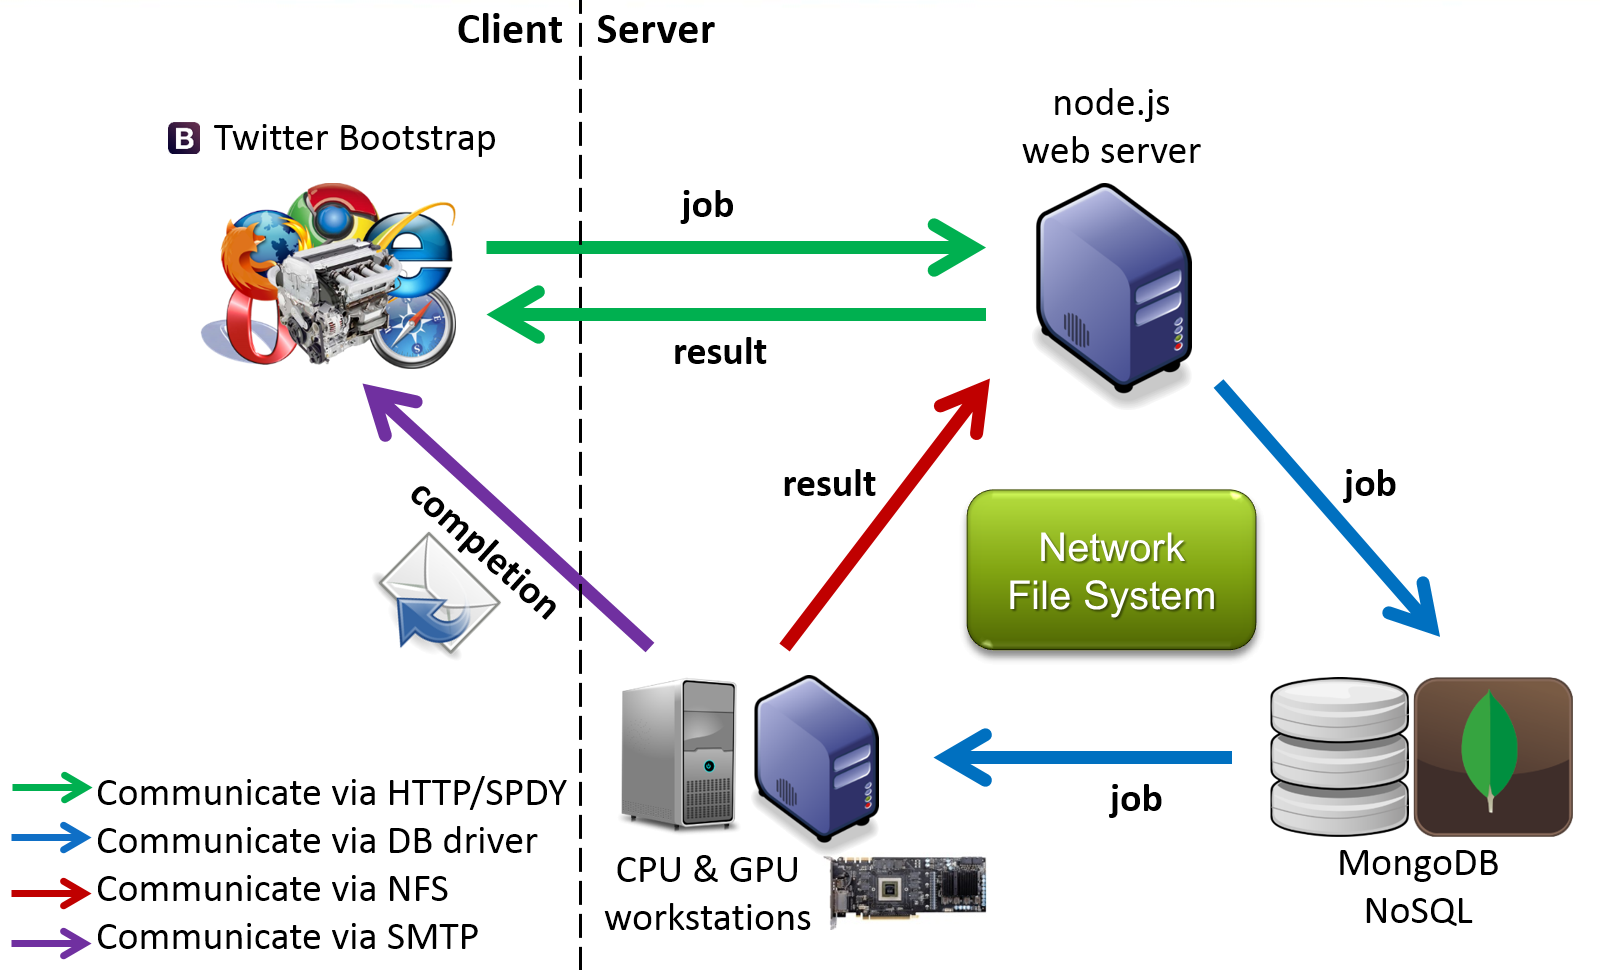
\includegraphics[width=\linewidth,keepaspectratio=true]{../istar/Architecture.eps}
\caption{\label{architecture} The istar architecture.}
\end{center}
\end{figure}

\clearpage

\begin{figure}
\begin{center}
%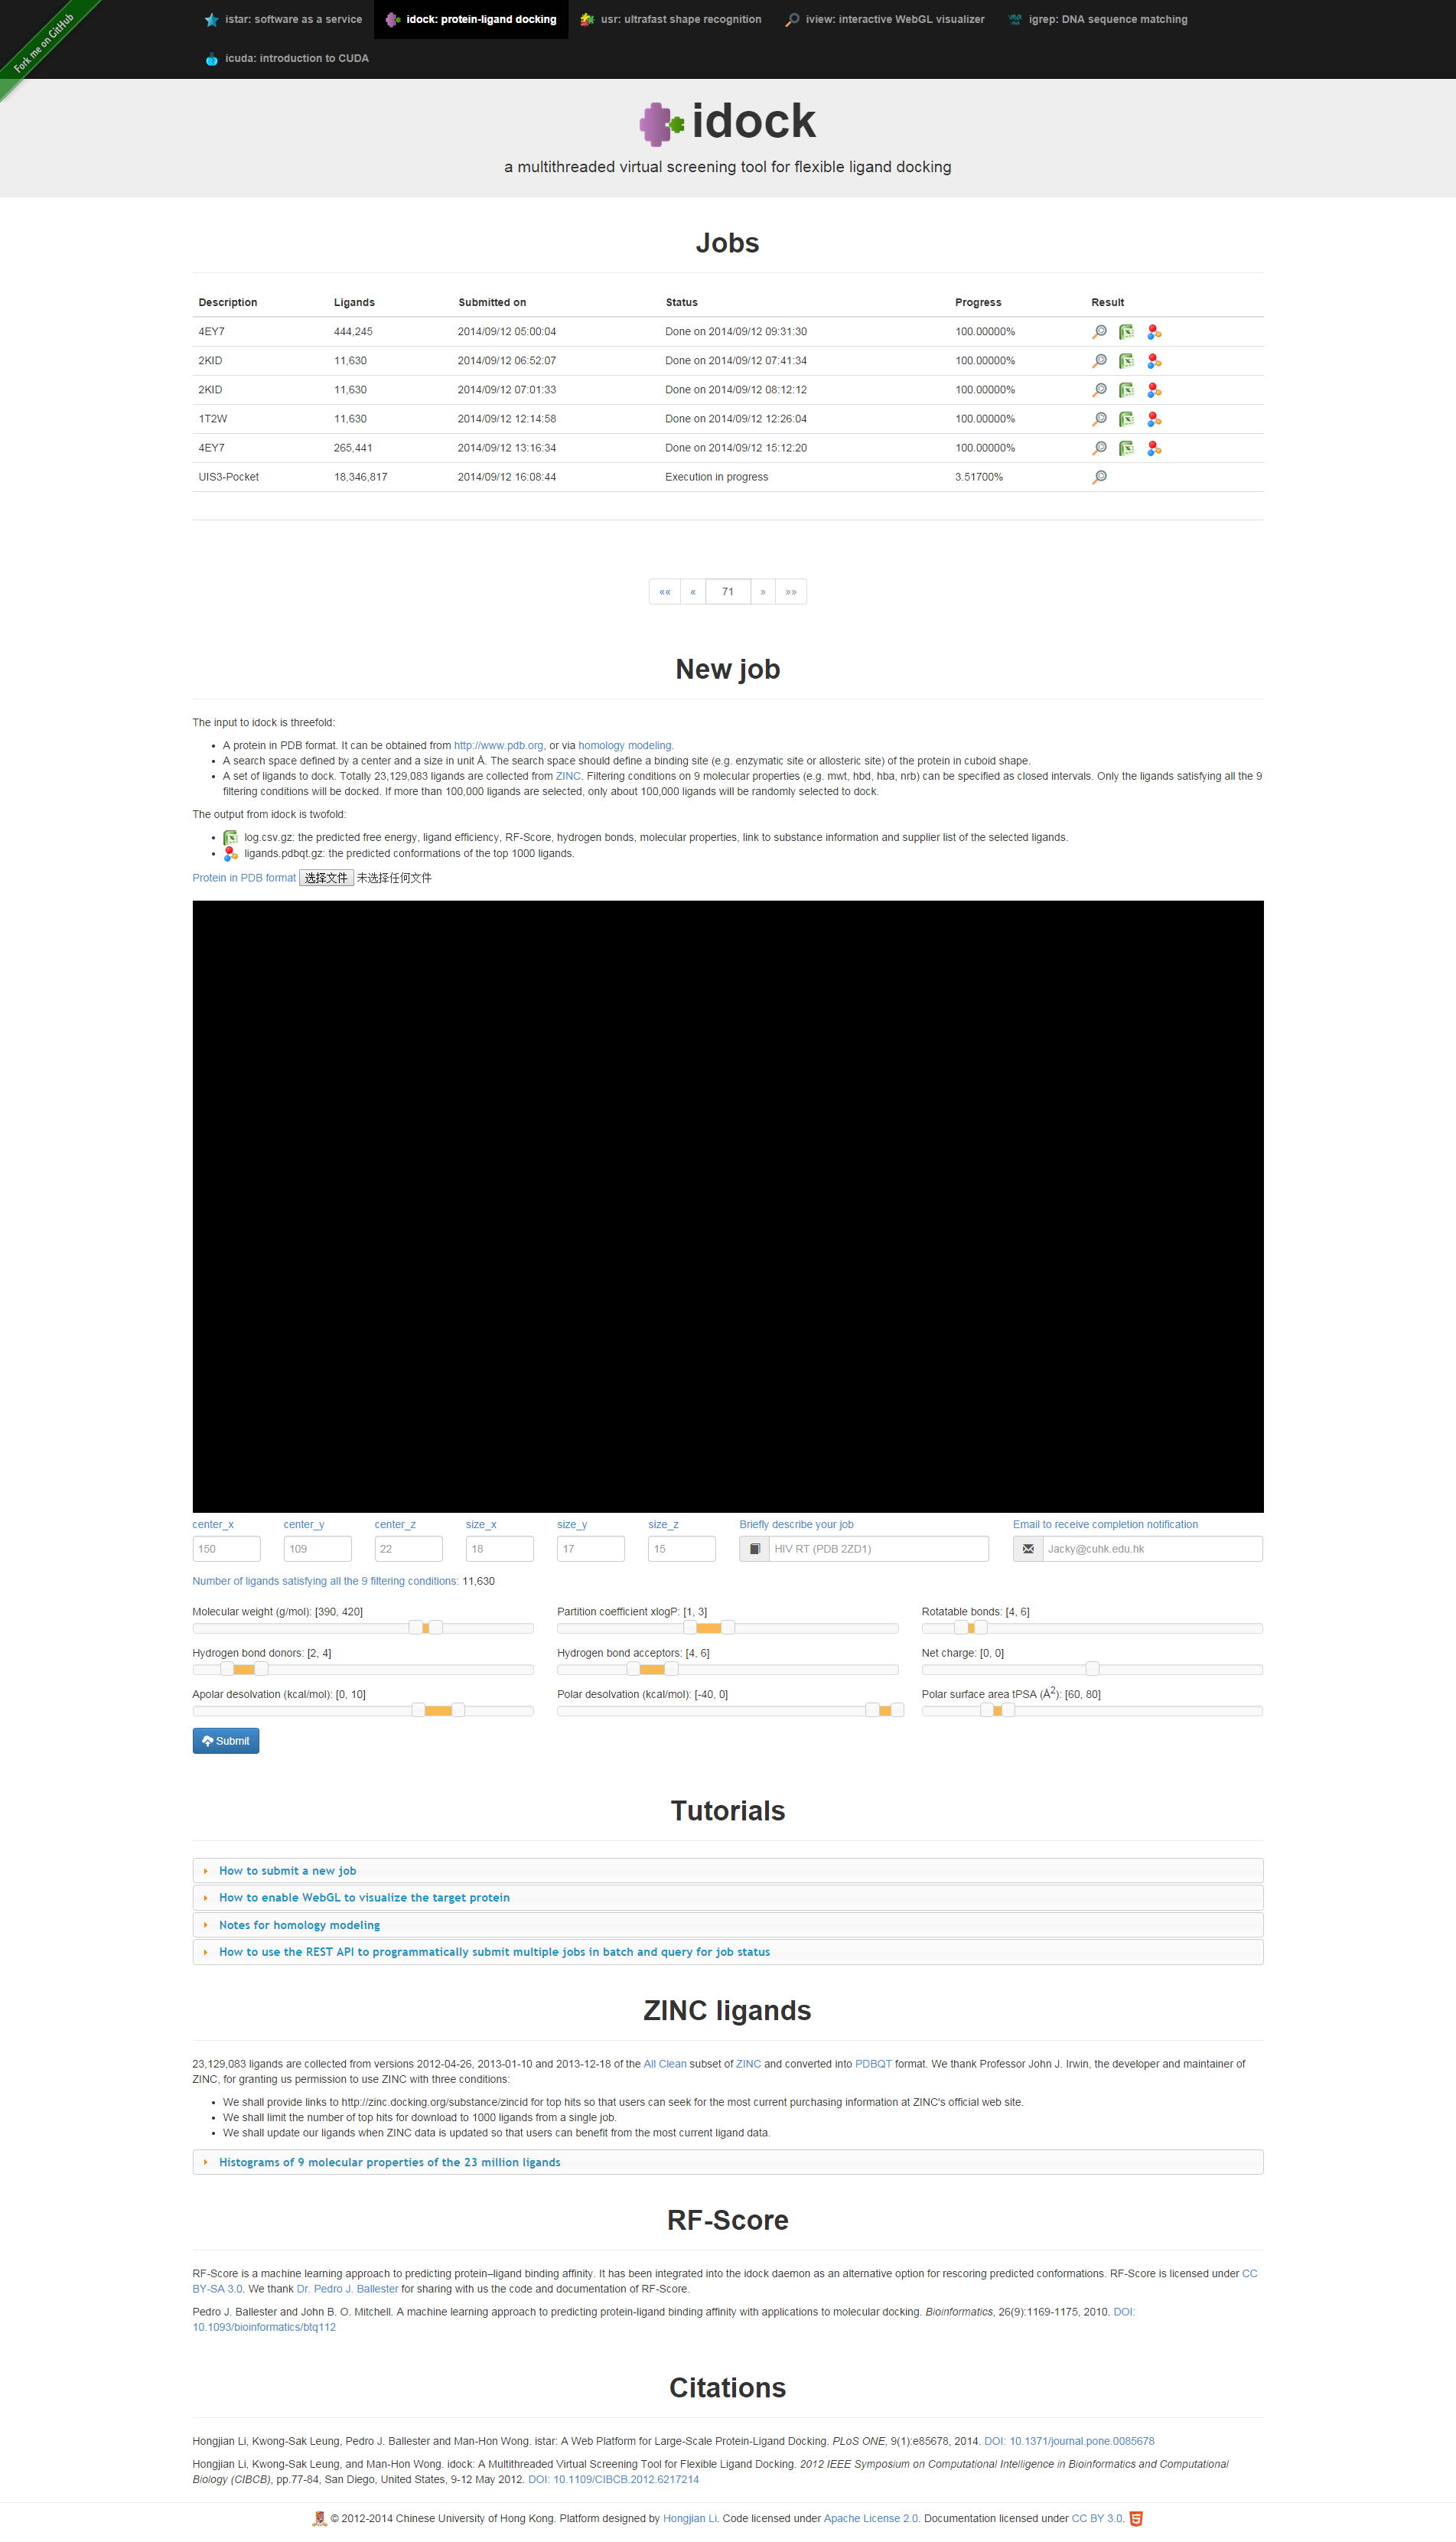
\includegraphics[width=0.9\linewidth,keepaspectratio=true]{../istar/idock.eps}
\caption{\label{idock} The idock web site on istar, available at http://idock.cse.cuhk.edu.hk}
\end{center}
\end{figure}

\clearpage

\begin{center}
\begin{figure}
\subfloat
{
%  \includegraphics[width=0.315\linewidth]{../istar/mwt.eps}
}
\subfloat
{
%  \includegraphics[width=0.315\linewidth]{../istar/logp.eps}
}
\subfloat
{
%  \includegraphics[width=0.315\linewidth]{../istar/ad.eps}
}
\\
\subfloat
{
%  \includegraphics[width=0.315\linewidth]{../istar/pd.eps}
}
\subfloat
{
%  \includegraphics[width=0.315\linewidth]{../istar/hbd.eps}
}
\subfloat
{
%  \includegraphics[width=0.315\linewidth]{../istar/hba.eps}
}
\\
\subfloat
{
%  \includegraphics[width=0.315\linewidth]{../istar/tpsa.eps}
}
\subfloat
{
%  \includegraphics[width=0.315\linewidth]{../istar/charge.eps}
}
\subfloat
{
%  \includegraphics[width=0.315\linewidth]{../istar/nrb.eps}
}
\caption{\label{LigandProperties} Histogram distributions of 9 molecular properties of the 12,171,187 clean ligands.}
\end{figure}
\end{center}

\clearpage

\begin{figure}
\begin{center}
%\includegraphics[width=\linewidth,keepaspectratio=true]{../istar/2PhaseDocking.eps}
\caption{\label{2PhaseDocking} Illustration of 2-phase docking.}
\end{center}
\end{figure}

\clearpage

\begin{center}
\begin{figure}
\centering
\subfloat[Job-level parallelism.]
{
%  \includegraphics[width=\linewidth]{../istar/JobLevelParallelism.eps}
}
\\
\subfloat[Slice-level parallelism.]
{
%  \includegraphics[width=\linewidth]{../istar/SliceLevelParallelism.eps}
}
\caption{\label{2LevelParallelism} Illustration of 2-level parallelism.}
\end{figure}
\end{center}

\clearpage

\begin{figure}
\begin{center}
\includegraphics[width=\linewidth,keepaspectratio=true]{../istar/OutputPDBQT.eps}
\caption{\label{OutputPDBQT} Verbose output of the idock daemon in PDBQT format.}
\end{center}
\end{figure}

\clearpage

\begin{figure}
\begin{center}
\includegraphics[width=\linewidth,keepaspectratio=true]{../istar/OutputCSV.eps}
\caption{\label{OutputCSV} Summary output of the idock daemon in CSV format.}
\end{center}
\end{figure}

\clearpage

\begin{figure}
\begin{center}
%\includegraphics[width=\linewidth]{../istar/ThreadPool.eps}
\caption{A thread pool of four threads competing for tasks. X: executed task. R: running task. Q: queued task.}
\label{ThreadPool}
\end{center}
\end{figure}

\clearpage

\begin{figure}
\begin{center}
%\includegraphics[width=\linewidth]{../istar/Compression.eps}
\caption{Gzip/Bzip2 compression/decompression support.}
\label{Compression}
\end{center}
\end{figure}

\clearpage

\begin{figure}
\begin{center}
%\includegraphics[width=\linewidth]{../istar/ChemicalElements.eps}
\caption{Chemical elements in red box are supported by both Vina and idock. Chemical elements in blue box are additional chemical elements solely supported by idock.}
\label{ChemicalElements}
\end{center}
\end{figure}

\clearpage

\begin{center}
\begin{figure}
\subfloat[PDB ID 1B8N. Vina RMSD1 = 0.139 \AA. idock RMSD1 = 0.127 \AA.]
{
  \includegraphics[width=0.485\linewidth]{../istar/Redocking1B8N.eps}
}
\subfloat[PDB ID 4TMN. Vina RMSD1 = 8.401 \AA. idock RMSD1 = 9.909 \AA.]
{
  \includegraphics[width=0.485\linewidth]{../istar/Redocking4TMN.eps}
}
\\
\subfloat[PDB ID 1PKX. Vina RMSD1 = 7.059 \AA. idock RMSD1 = 0.214 \AA.]
{
  \includegraphics[width=0.485\linewidth]{../istar/Redocking1PKX.eps}
}
\subfloat[PDB ID 3HV8. Vina RMSD1 = 0.290 \AA. idock RMSD1 = 10.232 \AA.]
{
  \includegraphics[width=0.485\linewidth]{../istar/Redocking3HV8.eps}
}
\caption{\label{Redocking} Redocking results of four cases.}
\end{figure}
\end{center}

\clearpage

\begin{table}
\centering
\begin{tabular}{lrrrrrr}
\hline
& \multicolumn{2}{c}{PDBbind v2012} & \multicolumn{2}{c}{PDBbind v2011} & \multicolumn{2}{c}{CSAR NRC HiQ}\\
Condition & idock & Vina & idock & Vina & idock & Vina\\
\hline
RMSD1 = RMSDm & 49\% & 53\% & 47\% & 54\% & 57\% & 71\%\\
RMSD2 = RMSDm & 15\% & 16\% & 16\% & 14\% & 17\% & 13\%\\
RMSD3 = RMSDm &  8\% &  7\% &  8\% &  8\% &  7\% &  4\%\\
RMSD4 = RMSDm &  6\% &  6\% &  6\% &  5\% &  5\% &  3\%\\
RMSD5 = RMSDm &  5\% &  4\% &  5\% &  5\% &  4\% &  1\%\\
RMSD6 = RMSDm &  5\% &  3\% &  5\% &  4\% &  3\% &  3\%\\
RMSD7 = RMSDm &  4\% &  4\% &  5\% &  4\% &  1\% &  2\%\\
RMSD8 = RMSDm &  5\% &  3\% &  4\% &  3\% &  3\% &  2\%\\
RMSD9 = RMSDm &  4\% &  3\% &  4\% &  3\% &  3\% &  2\%\\
\noalign{\smallskip}
RMSD1 \textless\ 0.5 \AA & 10\% & 12\% & 11\% & 12\% & 21\% & 21\%\\
RMSD1 \textless\ 1.0 \AA & 26\% & 31\% & 29\% & 31\% & 40\% & 47\%\\
RMSD1 \textless\ 1.5 \AA & 43\% & 47\% & 45\% & 47\% & 61\% & 67\%\\
RMSD1 \textless\ 2.0 \AA & 51\% & 56\% & 53\% & 56\% & 68\% & 73\%\\
RMSD1 \textless\ 2.5 \AA & 56\% & 61\% & 58\% & 61\% & 72\% & 76\%\\
\noalign{\smallskip}
RMSDm \textless\ 0.5 \AA & 12\% & 15\% & 14\% & 15\% & 24\% & 26\%\\
RMSDm \textless\ 1.0 \AA & 35\% & 40\% & 39\% & 40\% & 54\% & 55\%\\
RMSDm \textless\ 1.5 \AA & 61\% & 65\% & 64\% & 65\% & 78\% & 84\%\\
RMSDm \textless\ 2.0 \AA & 72\% & 79\% & 74\% & 78\% & 86\% & 92\%\\
RMSDm \textless\ 2.5 \AA & 77\% & 85\% & 79\% & 84\% & 90\% & 94\%\\
\hline
\end{tabular}
\caption{\label{SuccessRate} Redocking success rates of idock and AutoDock Vina on PDBbind v2012 and v2011 and CSAR NRC HiQ Set 24Sept2010 under various conditions regarding the RMSD (Root Mean Square Deviation) values between the crystal and docked conformations.}
\end{table}

\clearpage

\begin{center}
\begin{figure}
\subfloat[PDBbind v2012 refined set]
{
%  \includegraphics[width=0.31\linewidth]{../istar/PDBbind2012FECorrelation.eps}
}
\subfloat[PDBbind v2011 refined set]
{
%  \includegraphics[width=0.31\linewidth]{../istar/PDBbind2011FECorrelation.eps}
}
\subfloat[CSAR NRC HiQ Set 24Sept2010]
{
%  \includegraphics[width=0.31\linewidth]{../istar/CSARFECorrelation.eps}
}
\caption{\label{FECorrelation} Binding affinity correlation on PDBbind v2012 and v2011 and CSAR NRC HiQ Set 24Sept2010. Along the diagonal from top left to bottom right are the histogram distributions of experimental binding affinities, binding affinities predicted by AutoDock Vina, and binding affinities predicted by idock.}
\end{figure}
\end{center}

\clearpage

\begin{center}
\begin{figure}
\subfloat
{
  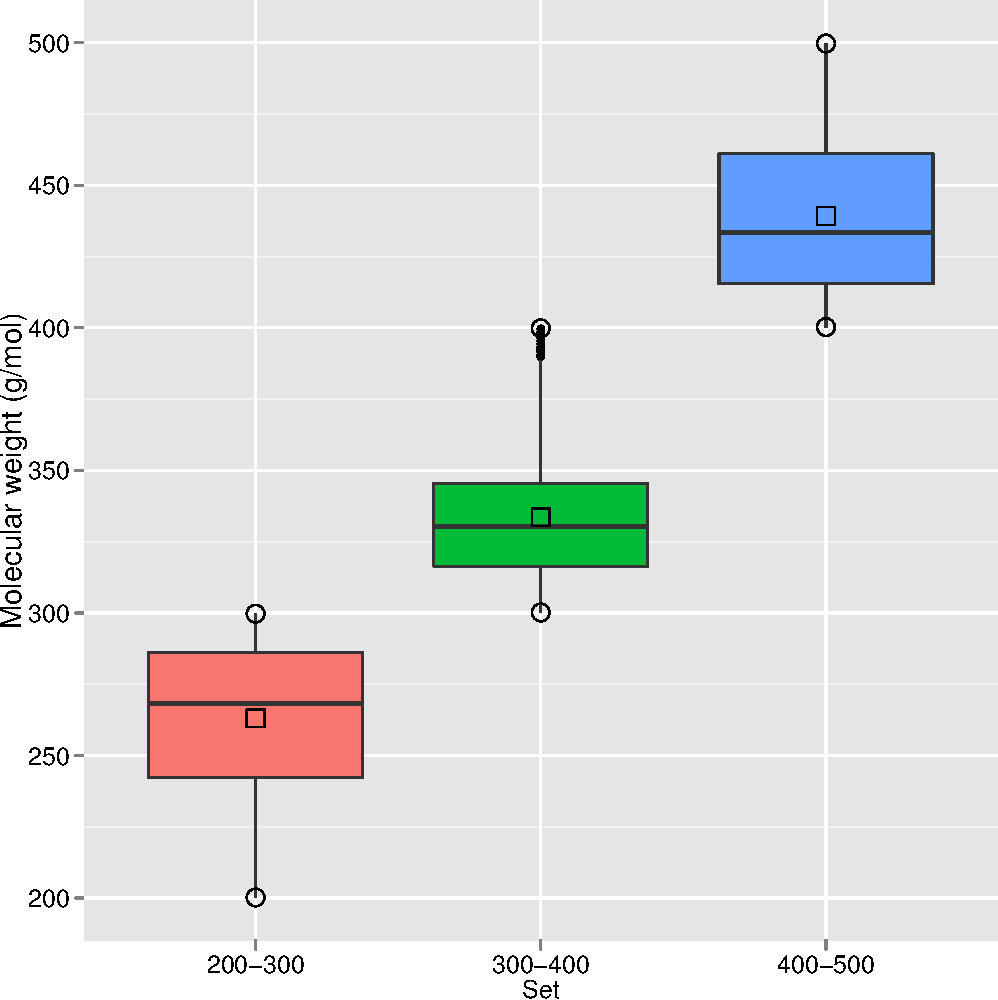
\includegraphics[width=0.485\linewidth]{../istar/MWT3.eps}
}
\subfloat
{
  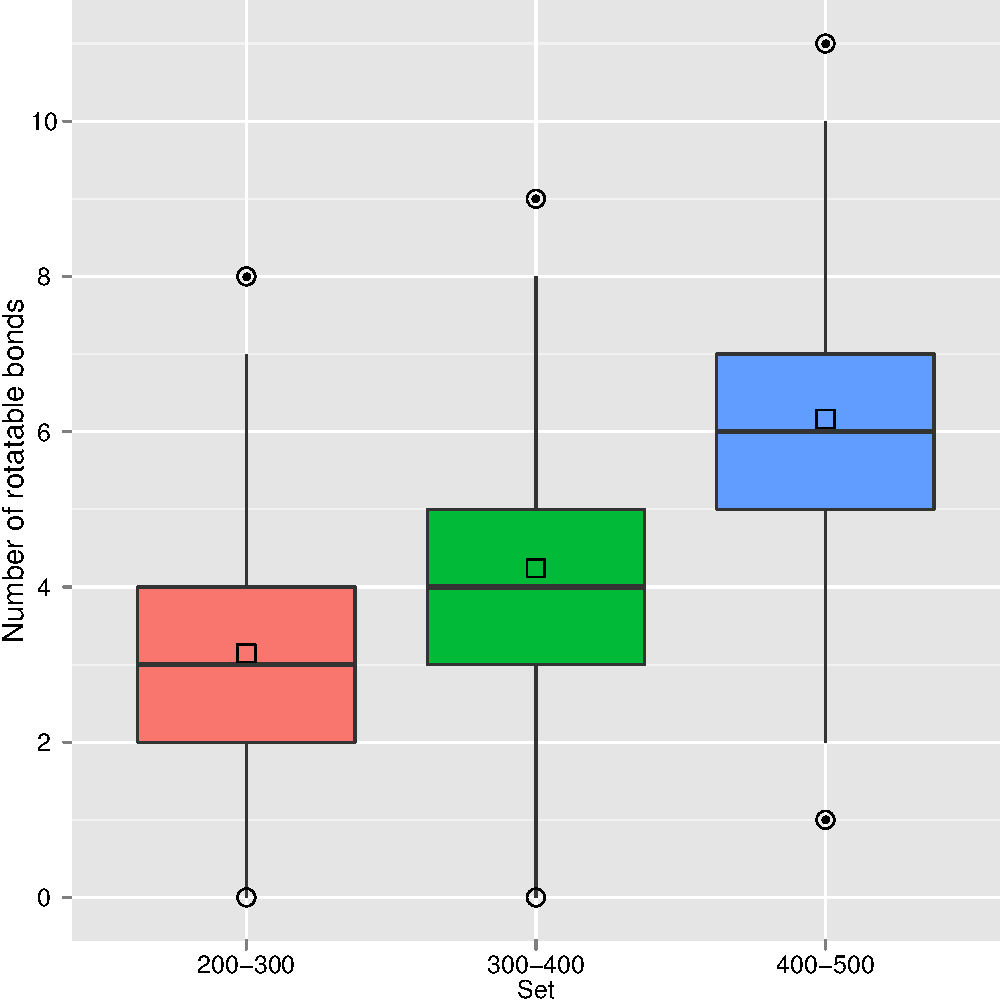
\includegraphics[width=0.485\linewidth]{../istar/NRB3.eps}
}
\caption{\label{MWT-NRB} Boxplot of molecular weight and number of rotatable bonds of the 1000 ligands of each of the three molecular weight sets.}
\end{figure}
\end{center}

\clearpage

\begin{longtable}{crrrrrr}
\hline
& \multicolumn{2}{c}{200-300g/mol} & \multicolumn{2}{c}{300-400g/mol} & \multicolumn{2}{c}{400-500g/mol}\\
& CPU & Elapsed & CPU & Elapsed & CPU & Elapsed\\
\hline
\multicolumn{7}{l}{\textbf{1HCL} human cyclin-dependent kinase 2}\\
Vina  & 12.57 &  3.33 & 22.55 &  5.91 & 51.62 & 13.41\\
idock &  0.63 &  0.16 &  0.92 &  0.24 &  1.38 &  0.36\\
\multicolumn{7}{l}{\textbf{1J1B} human tau protein kinase I}\\
Vina  &  9.07 &  2.47 & 14.69 &  3.92 & 32.28 &  8.49\\
idock &  0.78 &  0.21 &  1.25 &  0.33 &  2.35 &  0.62\\
\multicolumn{7}{l}{\textbf{1LI4} human S-adenosylhomocysteine hydrolase}\\
Vina  & 11.82 &  3.30 & 19.08 &  5.22 & 39.41 & 10.64\\
idock &  0.89 &  0.23 &  1.55 &  0.40 &  3.15 &  0.82\\
\multicolumn{7}{l}{\textbf{1V9U} human rhinovirus 2 coat protein VP1}\\
Vina  &  9.80 &  2.95 & 15.55 &  4.62 & 29.75 &  8.49\\
idock &  0.97 &  0.25 &  1.64 &  0.42 &  3.42 &  0.89\\
\multicolumn{7}{l}{\textbf{2IQH} influenza A virus nucleoprotein NP}\\
Vina  &  9.51 &  2.66 & 15.03 &  4.08 & 29.64 &  7.83\\
idock &  0.92 &  0.24 &  1.59 &  0.41 &  3.41 &  0.88\\
\multicolumn{7}{l}{\textbf{2XSK} Escherichia coli curli protein CsgC - SeCys}\\
Vina  & 10.44 &  2.71 & 17.89 &  4.61 & 40.58 & 10.41\\
idock &  0.71 &  0.19 &  1.16 &  0.30 &  2.16 &  0.56\\
\multicolumn{7}{l}{\textbf{2ZD1} HIV-1 reverse transcriptase}\\
Vina  &  9.78 &  2.70 & 17.67 &  4.76 & 42.03 & 11.33\\
idock &  0.97 &  0.25 &  1.52 &  0.39 &  2.60 &  0.69\\
\multicolumn{7}{l}{\textbf{2ZNL} influenza virus RNA polymerase subunit PA}\\
Vina  &  9.49 &  2.60 & 15.04 &  4.01 & 29.97 &  7.82\\
idock &  0.89 &  0.23 &  1.56 &  0.40 &  3.41 &  0.87\\
\multicolumn{7}{l}{\textbf{3BGS} human purine nucleoside phosphorylase}\\
Vina  &  9.59 &  2.57 & 16.50 &  4.37 & 38.42 & 10.14\\
idock &  0.95 &  0.25 &  1.55 &  0.40 &  2.81 &  0.74\\
\multicolumn{7}{l}{\textbf{3H0W} human S-adenosylmethionine decarboxylase}\\
Vina  &  9.85 &  2.64 & 17.67 &  4.70 & 41.69 & 11.04\\
idock &  0.88 &  0.23 &  1.35 &  0.35 &  2.20 &  0.58\\
\multicolumn{7}{l}{\textbf{3IAR} human adenosine deaminase}\\
Vina  & 11.25 &  3.03 & 20.21 &  5.39 & 46.93 & 12.53\\
idock &  0.80 &  0.21 &  1.21 &  0.32 &  2.01 &  0.53\\
\multicolumn{7}{l}{\textbf{3KFN} HIV protease}\\
Vina  & 10.53 &  2.80 & 18.37 &  4.83 & 42.43 & 11.03\\
idock &  0.77 &  0.20 &  1.20 &  0.32 &  2.09 &  0.55\\
\multicolumn{7}{l}{\textbf{Average across the above 12 receptors}}\\
Vina  & 10.31 &  2.81 & 17.52 &  4.70 & 38.73 & 10.26\\
idock &  0.85 &  0.22 &  1.38 &  0.36 &  2.58 &  0.67\\
\hline
\caption{\label{ExecutionTime} CPU time and elapsed time in hours of docking 3000 clean ligands of 3 molecular weight sets against 12 diverse receptors by AutoDock Vina and idock.}
\end{longtable}

\end{document}

